\section{Cloud Architecture and Design}

This system will be deployed using Infrastructure as a Service (IaaS) on Amazon Web Services (AWS).

\subsection{Cloud Provider Selection}
The growth in popularity of cloud services has fostered an industry with many competing cloud providers. Given the continued growth of the SmartV user-base, the choice to leverage an existing provider has been made to balance the increasing but dynamic demands of the platform while maintaining minimal-cost cloud infrastructure. Both internal and public cloud providers have been considered, including offerings from VMware, OpenStack, Azure, and Amazon Web Services (AWS).

The use of internal cloud provisioning necessitates a significant up-front cost in both the hardware and software required by the transition to cloud infrastructure, and is over-all less flexible than the infrastructure-as-a-service models provided by Azure and AWS. These caveats to an internal cloud deployment represent unnecessary additional costs and management responsibilities to SmartV, reducing the organisations focus on end-users.

For these reasons and over-all compatibility with the business requirements outlined in section \ref{sec:businessrequirements} AWS is selected as the cloud provider of choice for the project. The use of AWS also allows SmartV to bypass the upfront cost of any immediate upgrades to physical infrastructure by instead utilising storage, compute, and network provided by the AWS platform, paying for only the resources used by SmartV. The choice of AWS is also influenced by the ready availability of high-power compute instances required by the SmartV platform (see section \ref{sec:infrastructure-components}).

\subsection{Design Assumptions}

The preparation of this document makes a few key assumptions that will need to be confirmed with SmartV. These are the following: 

\begin{enumerate}
    \item \textbf{Provision of Software:} We assume SmartV has proprietary software suitable for serving the needs of its customer base, and is only looking to extend from an on-premises computing solution to a cloud infrastructure solution. No considertaion is made for changes to software not directly related to infrastructure.
    \item \textbf{Geographic Scope:} We assume SmartV operates primarily in the Asia-Pacific (APAC) region. We therefore design for traffic in the area by placing infrastructure primarily in Sydney datacentres, with high availability available in Singapore datacentres.
    \item \textbf{User Accounts:} We assume SmartV has interest in individual user profiles and accounts, which will need special consideration in this infrastructure environment to handle storage and backups.
    \item \textbf{Compute Requirements:} We assume SmartV is interested in high levels of compute. Video as a data source is an extremely large medium compared to, for e.g. text or music. Therefore we spec the compute capabilities quite highly, with support for high CPU, GPU, and RAM availability per instance.
\end{enumerate}

\subsection{Infrastructure Design}

\begin{figure}[H]\label{fig:awsdiagram}
    \centering
    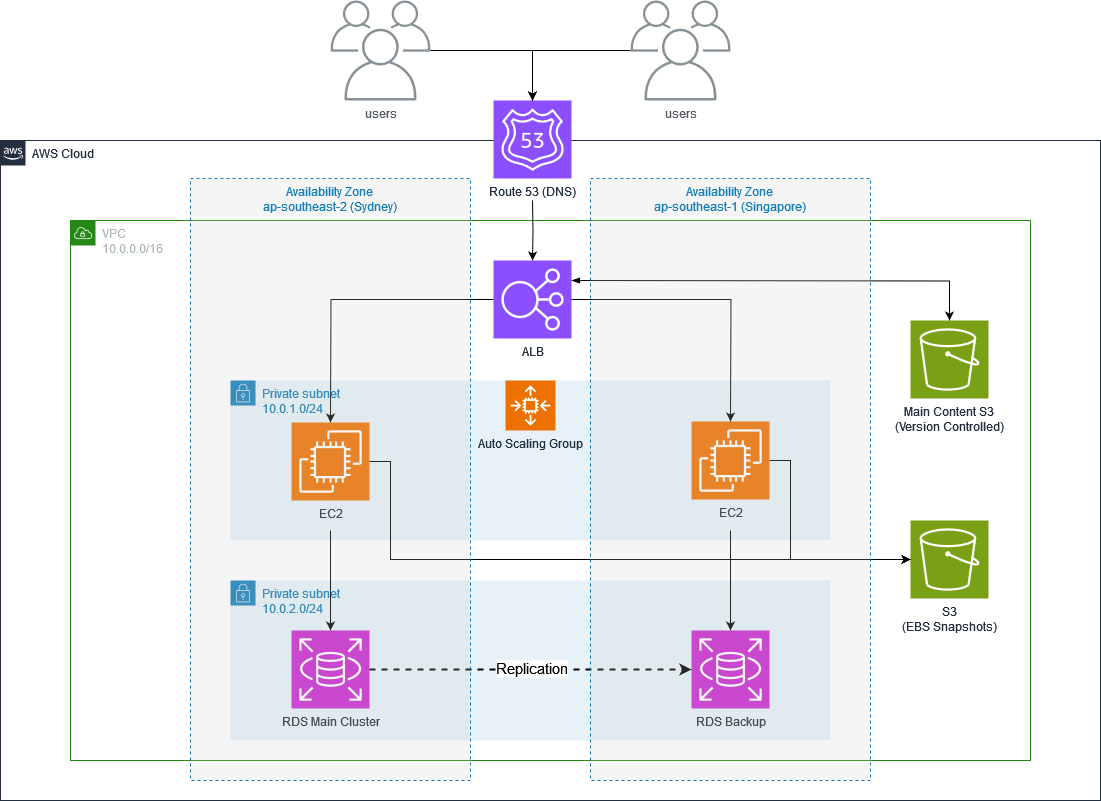
\includegraphics[width=\textwidth]{cci_aws}
    \caption{Cloud Infrastructure Topology}
\end{figure}

\subsection{Infrastructure Components}
\label{sec:infrastructure-components}

\subsubsection*{DNS (Route 53)}

Allowing global access through http, a DNS record is needed and will be achieved through an AWS Route 53 domain. This will transfer users to the ALB.

\subsubsection*{Network (ALB)}

To balance load across seperate compute clusters, an application load balancer (ALB) will handle distribution of incoming requests to allow transparent scaling of compute abstracted from the user, meaning bucekts of storage can scale infinitely.

\subsubsection*{Compute (EC2)}

Using an autoscaling group of EC2 instances of type ``p3.8xlarge'', compute will be handled and scaled with demand. The instance types are very large to accomodate for the intense RAM, CPU, and GPU requirements video demands. A key feature of S3 is the inherent scalability, as this is abstracted away from the end user. The use of this instance scale also allows networking performance of 10 Gbps. This will be very helpful as the most intense network requirements are occurring internally on AWS, between compute and content storage on S3.

\subsubsection*{Content Storage (S3)}

AWS Simple Storage Service (S3) allows for cheap and easy object storage through a HTTP API endpoint. This is suitable for storing the large files used by the service, and allowing avilability across the platform.

\subsubsection*{Backup Storage (S3)}

Snapshots of the drives associated with compute instances, the elastic block storage (EBS) drives, will be palced daily in a seperate S3 bucket to allow disaster recovery of user's work and files retained locally on the compute instance.

\subsubsection*{User Database (RDS)}

AWS Relational Database System (RDS) will be used to handle user information such as login, account details, and payment information. Using a traditional database system is suitable over S3 as it allows structure and replication.

\subsubsection*{Network (Public)}

The entire cloud system will exist within a private VPC, with the only publically exposed element being the ALB accessible through the Route 53 DNS record or associated IP address.

\subsubsection*{Network (Internal)}

Internally, the platform is networked through a private IPv4 subnet in CIDR block 10.0.0.0/16. Each private subnet in turn has it's own CIDR block with a netmask of 24. Compute and the RDS service reside in seperate private subnets to improve security.

\subsubsection*{Scaling (Compute)}

Using EC2 autoscaling groups, AWS will launch new compute instances as demand increases on pre-existing ones, placing them behind the ALB. Retaining a minimum of 1 instance ensures constant availability. An option available is keep ``warm pools'' of compute instances pre-initialized but not in use, allowing near instant upscaling as demand spikes.

\subsubsection*{High Availability}

High availability will be achieved through seperating cloud resources across two AWS availability zones (AZs), allowing an entire region of AWS to lose access, while maintaining service for customers. It also allows upgrades to infrastructure and software to cause a temporary planned outage in one region while maintaining uninterrupted service globally.

\subsection{Pricing}

Utilising scalable infrastructure as a service makes accurate, fixed estimations of costs difficult as prices are tied directly to utilisation. Here an estimate of month-to-month costs is provided as calculated via the AWS pricing calculator\footnote{See \url{https://calculator.aws}.}

% https://calculator.aws/#/addService
